\section{Durchführung}
Der Aufbau des Versuches wird in \autoref{fig:5} skizziert.
\begin{figure}[H] 
  \centering 
  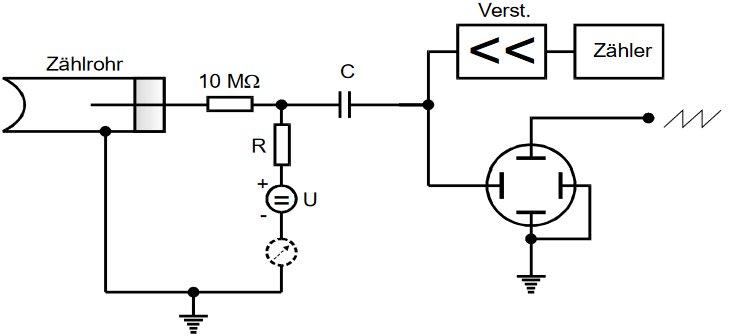
\includegraphics[width=9cm]{content/5.png} 
  \caption{Versuchsaufbau [1].} 
  \label{fig:5} 
\end{figure}
Es wird eine Probe vor das Myelarfenster gelegt und die Impulsrate in 120 Sekunden gemessen für den Spannungsbereich zwischen 330-700V in 10V-Schritten. Dazu wird der Strom gemessen, der vom Geiger-Müller-Zählrohr abfließt.\\
Für die Messung der Totzeit mit der Zwei-Quellen-Methode, wird erst eine Quelle gemssen, dann zwei Quellen und dann nur noch die zweite Quelle. Dabei werden wieder die Impulsraten zu 120 Sekunden gemessen.\\
Zusätzlich kann die Totzeit mit dem Oszilloskop gemessen werden, indem bei 330 V und 700 V die Abbildung des Oszilloskops mit \autoref{fig:3} verglichen wird [1]. 
